\documentclass[12pt, a4paper]{article}
\usepackage{../../../myconfig} % Gọi file cấu hình chuẩn myconfig.sty

% ==========================================
% BẮT ĐẦU NỘI DUNG TÀI LIỆU - ĐỀ SỐ 3
% ==========================================
\begin{document}

% Tiêu đề đầu đề thi: {Nhãn cam} {Chữ to chính giữa} {Chữ ở góc phải Header}
\titlebox{ĐỀ SỐ 3}{ĐỀ THI GIỮA HỌC KỲ I}{Ôn tập GKI}

\textit{\textbf{PHẦN I. Câu trắc nghiệm nhiều phương án lựa chọn. Thí sinh trả lời từ Câu 1 đến Câu 12. Mỗi câu hỏi thí sinh chỉ chọn một phương án.}}

\vspace{0.3cm}

% --- CÂU 1 ---
\questionLinesManual{0}{1}{Đường cong trong hình vẽ dưới đây là đồ thị của hàm số nào sau đây?
\begin{center}
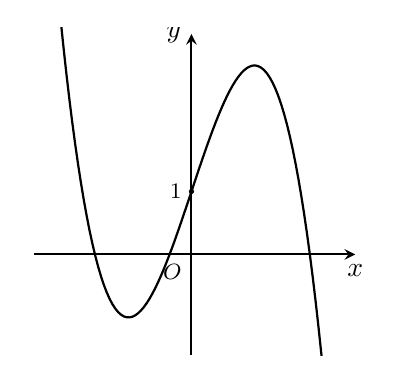
\begin{tikzpicture}[scale=0.8, >=stealth]
    \clip (-2.6, -1.6) rectangle (2.8, 3.6);
    \draw[->, line width=0.7pt] (-2.5, 0) -- (2.6, 0) node[below] {$x$};
    \draw[->, line width=0.7pt] (0, -1.6) -- (0, 3.5) node[left] {$y$};
    \node[below left, font=\footnotesize] at (0, 0) {$O$};
    \fill (0, 1) circle (1.2pt) node[left, font=\footnotesize] {$1$};
    % Đồ thị bậc 3: y = -x^3 + 3x + 1
    \draw[thick, domain=-2.3:2.2, samples=100] plot (\x, {-(\x)^3 + 3*(\x) + 1});
\end{tikzpicture}
\end{center}
}{%
    \begin{tasks}(2)
        \task $y = x^3 - 3x + 1$.
        \task $y = -x^4 + x^2 - 1$.
        \task $y = -x^3 + 3x + 1$.
        \task $y = -x^2 + 2x + 1$.
    \end{tasks}
}

% --- CÂU 2 ---
\questionLinesManual{0}{2}{Cho hàm số $y=f(x)$ xác định và liên tục trên khoảng $(-\infty;+\infty)$, có bảng biến thiên như hình vẽ dưới đây:
\begin{center}

\begin{tikzpicture}[scale=0.95]
    \tkzTabInit[lgt=1.2, espcl=2.2, deltacl=0.5]{$x$/0.8, $y'$/0.7, $y$/1.8}{$-\infty$, $-1$, $1$, $+\infty$}
    \tkzTabLine{, -, 0, +, 0, -, }
    \tkzTabVar{+/$+\infty$, -/$-1$, +/$3$, -/$-\infty$}
\end{tikzpicture}
\end{center}
Mệnh đề nào sau đây là mệnh đề đúng?}{%
    \begin{tasks}(2)
        \task Hàm số nghịch biến trên khoảng $(-\infty;1)$.
        \task Hàm số nghịch biến trên khoảng $(1;+\infty)$.
        \task Hàm số nghịch biến trên khoảng $(-1;3)$.
        \task Hàm số nghịch biến trên khoảng $(-1;+\infty)$.
    \end{tasks}
}

% --- CÂU 3 ---
\questionLinesManual{0}{3}{Cho hàm số $y=f(x)$ liên tục trên $\mathbb{R}$ và có đồ thị như hình vẽ. Số điểm cực trị của hàm số là
\begin{center}
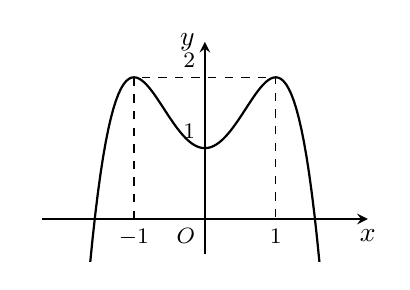
\begin{tikzpicture}[scale=0.9, >=stealth]
    \clip (-2.5, -0.6) rectangle (2.5, 2.7);
    \draw[->, line width=0.7pt] (-2.3, 0) -- (2.3, 0) node[below] {$x$};
    \draw[->, line width=0.7pt] (0, -0.5) -- (0, 2.5) node[left] {$y$};
    \node[below left, font=\footnotesize] at (0, 0) {$O$};
    
    % Đường dóng cực đại
    \draw[dashed, line width=0.5pt] (-1, 0) -- (-1, 2) -- (1, 2) -- (1, 0);
    \node[below, font=\footnotesize] at (-1, 0) {$-1$};
    \node[below, font=\footnotesize] at (1, 0) {$1$};
    \node[above left, font=\footnotesize] at (0, 2) {$2$};
    \node[above left, font=\footnotesize] at (0, 1) {$1$};
    
    % Hàm trùng phương y = -x^4 + 2x^2 + 1
    \draw[thick, domain=-1.8:1.8, samples=100] plot (\x, {-(\x)^4 + 2*(\x)^2 + 1});
\end{tikzpicture}
\end{center}
}{%
    \begin{tasks}(4)
        \task $2$.
        \task $4$.
        \task $3$.
        \task $1$.
    \end{tasks}
}

% --- CÂU 4 ---
\questionLinesManual{0}{4}{Cho hàm số $y=f(x)$ liên tục trên đoạn $[-1;3]$ có đồ thị như hình vẽ. Gọi $M$ và $m$ lần lượt là giá trị lớn nhất, giá trị nhỏ nhất của hàm số đã cho trên đoạn $[-1;3]$. Giá trị của $M+m$ bằng
\begin{center}
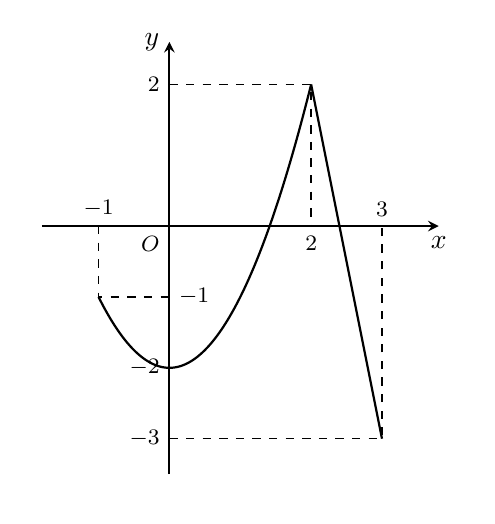
\begin{tikzpicture}[scale=0.9, >=stealth]
    \clip (-2.0, -3.8) rectangle (4.2, 2.8);
    \draw[->, line width=0.7pt] (-1.8, 0) -- (3.8, 0) node[below] {$x$};
    \draw[->, line width=0.7pt] (0, -3.5) -- (0, 2.6) node[left] {$y$};
    \node[below left, font=\footnotesize] at (0, 0) {$O$};

    % Các đường dóng
    \draw[dashed, line width=0.5pt] (-1, 0) -- (-1, -1) -- (0, -1);
    \draw[dashed, line width=0.5pt] (0, 2) -- (2, 2) -- (2, 0);
    \draw[dashed, line width=0.5pt] (0, -3) -- (3, -3) -- (3, 0);

    \node[above, font=\footnotesize] at (-1, 0) {$-1$};
    \node[below, font=\footnotesize] at (2, 0) {$2$};
    \node[above, font=\footnotesize] at (3, 0) {$3$};
    \node[left, font=\footnotesize] at (0, 2) {$2$};
    \node[right, font=\footnotesize] at (0, -1) {$-1$};
    \node[left, font=\footnotesize] at (0, -2) {$-2$};
    \node[left, font=\footnotesize] at (0, -3) {$-3$};

    % Đồ thị gồm cung parabol từ [-1; 2] và đoạn thẳng từ [2; 3]
    \draw[thick, domain=-1:2, samples=100] plot (\x, {(\x)^2 - 2});
    \draw[thick] (2, 2) -- (3, -3);
\end{tikzpicture}
\end{center}
}{%
    \begin{tasks}(2)
        \task $M+m=3$.
        \task $M+m=0$.
        \task $M+m=-1$.
        \task $M+m=5$.
    \end{tasks}
}

% --- CÂU 5 ---
\questionLinesManual{0}{5}{Hàm số $y=-x^3+x^2+5x-5$ đạt cực tiểu tại điểm $x_0$. Giá trị cực tiểu $y_0$ là}{%
    \begin{tasks}(4)
        \task $y_0=-8$.
        \task $y_0=\dfrac{5}{3}$.
        \task $y_0=-1$.
        \task $y_0=\dfrac{40}{27}$.
    \end{tasks}
}

% --- CÂU 6 ---
\questionLinesManual{0}{6}{Cho hai vectơ $\vec{a}$ và $\vec{b}$ thỏa mãn $|\vec{a}|=3$, $|\vec{b}|=2$ và $(\vec{a},\vec{b})=60^{\circ}$. Tích vô hướng $\vec{a}\cdot\vec{b}$ bằng}{%
    \begin{tasks}(4)
        \task $\vec{a}\cdot\vec{b}=3$.
        \task $\vec{a}\cdot\vec{b}=3\sqrt{3}$.
        \task $\vec{a}\cdot\vec{b}=6$.
        \task $\vec{a}\cdot\vec{b}=12$.
    \end{tasks}
}

% --- CÂU 7 ---
\questionLinesManual{0}{7}{Biết hàm số $y=\dfrac{ax+1}{x-b}$ có đồ thị như hình vẽ sau. Hãy tìm giá trị thực của $a$ và $b$.
\begin{center}
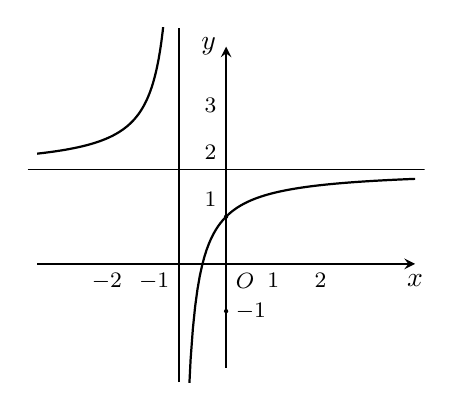
\begin{tikzpicture}[scale=0.6, >=stealth]
    \clip (-4.2, -2.5) rectangle (4.2, 5.0);
    \draw[->, line width=0.7pt] (-4.0, 0) -- (4.0, 0) node[below] {$x$};
    \draw[->, line width=0.7pt] (0, -2.2) -- (0, 4.6) node[left] {$y$};
    \node[below right, font=\footnotesize] at (0, 0) {$O$};

    % Tiệm cận đứng x = -1, tiệm cận ngang y = 2
    \draw[line width=0.6pt] (-1, -2.5) -- (-1, 5.0);
    \draw[line width=0.6pt] (-4.2, 2) -- (4.2, 2);

    \node[below left, font=\footnotesize] at (-1, 0) {$-1$};
    \node[below left, font=\footnotesize] at (-2, 0) {$-2$};
    \node[below, font=\footnotesize] at (1, 0) {$1$};
    \node[below, font=\footnotesize] at (2, 0) {$2$};
    \node[above left, font=\footnotesize] at (0, 2) {$2$};
    \node[above left, font=\footnotesize] at (0, 3) {$3$};

    % Giao điểm Oy (0; 1) và điểm (-0.5; 0)
    \fill (0, 1) circle (1.3pt) node[above left, font=\footnotesize] {$1$};
    \fill (0, -1) circle (1.3pt) node[right, font=\footnotesize] {$-1$};

    % Đồ thị: y = (2x + 1)/(x + 1) -> a = 2, b = -1
    \draw[thick, domain=-4.0:-1.2, samples=100] plot (\x, {(2*(\x)+1)/((\x)+1)});
    \draw[thick, domain=-0.8:4.0, samples=100] plot (\x, {(2*(\x)+1)/((\x)+1)});
\end{tikzpicture}
\end{center}
}{%
    \begin{tasks}(2)
        \task $a=2$ và $b=-1$.
        \task $a=-1$ và $b=2$.
        \task $a=1$ và $b=-2$.
        \task $a=-2$ và $b=1$.
    \end{tasks}
}

% --- CÂU 8 ---
\questionLinesManual{0}{8}{Giá trị nhỏ nhất của hàm số $f(x)=xe^x$ trên đoạn $[1;5]$ là}{%
    \begin{tasks}(4)
        \task $5e^5$.
        \task $-\dfrac{1}{e}$.
        \task $1$.
        \task $e$.
    \end{tasks}
}

% --- CÂU 9 ---
\questionLinesManual{0}{9}{Đường tiệm cận xiên của đồ thị hàm số $y=\dfrac{x^2+2x-3}{x-2}$ là đường thẳng có phương trình nào dưới đây?}{%
    \begin{tasks}(4)
        \task $y=x+1$.
        \task $y=x+4$.
        \task $y=x-4$.
        \task $y=x-2$.
    \end{tasks}
}

% --- CÂU 10 ---
\questionLinesManual{0}{10}{Cho hình lập phương $ABCD.A'B'C'D'$ có cạnh bằng $a$. Góc giữa hai vectơ $\vec{AC}$ và $\vec{B'D'}$ bằng
\begin{center}
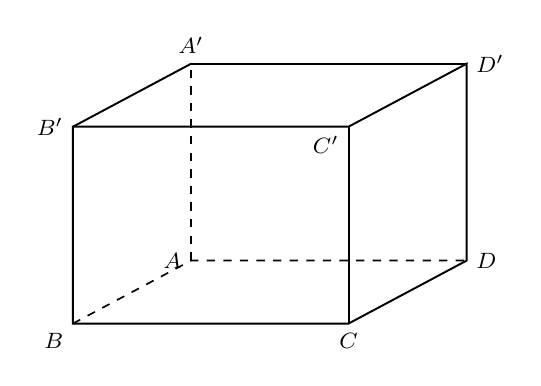
\begin{tikzpicture}[scale=1, >=stealth]
    \coordinate (A) at (1.5, 0.8);
    \coordinate (B) at (0, 0);
    \coordinate (C) at (3.5, 0);
    \coordinate (D) at (5, 0.8);
    
    \coordinate (A') at (1.5, 3.3);
    \coordinate (B') at (0, 2.5);
    \coordinate (C') at (3.5, 2.5);
    \coordinate (D') at (5, 3.3);

    % Nét đứt
    \draw[dashed, line width=0.6pt] (B) -- (A) -- (D);
    \draw[dashed, line width=0.6pt] (A) -- (A');

    % Nét liền
    \draw[line width=0.7pt] (B) -- (C) -- (D) -- (D') -- (C') -- (B') -- cycle;
    \draw[line width=0.7pt] (A') -- (B');
    \draw[line width=0.7pt] (A') -- (D');
    \draw[line width=0.7pt] (C) -- (C');

    % Tên đỉnh
    \node[left, font=\footnotesize] at (A) {$A$};
    \node[below left, font=\footnotesize] at (B) {$B$};
    \node[below, font=\footnotesize] at (C) {$C$};
    \node[right, font=\footnotesize] at (D) {$D$};
    \node[above, font=\footnotesize] at (A') {$A'$};
    \node[left, font=\footnotesize] at (B') {$B'$};
    \node[below left, font=\footnotesize] at (C') {$C'$};
    \node[right, font=\footnotesize] at (D') {$D'$};
\end{tikzpicture}
\end{center}
}{%
    \begin{tasks}(4)
        \task $90^{\circ}$.
        \task $135^{\circ}$.
        \task $60^{\circ}$.
        \task $45^{\circ}$.
    \end{tasks}
}

% --- CÂU 11 ---
\questionLinesManual{0}{11}{Cho hình lập phương $ABCD.A'B'C'D'$ có cạnh bằng $a$. Độ dài của vectơ $\vec{u}=\vec{AB}+\vec{AD}-\vec{AA'}$ bằng}{%
    \begin{tasks}(4)
        \task $|\vec{u}|=a$.
        \task $|\vec{u}|=a\sqrt{3}$.
        \task $|\vec{u}|=a\sqrt{2}$.
        \task $|\vec{u}|=3a$.
    \end{tasks}
}

% --- CÂU 12 ---
\questionLinesManual{0}{12}{Tìm điều kiện của tham số $m$ để hàm số $y=\dfrac{mx+5}{2x+1}$ đồng biến trên từng khoảng xác định của nó.}{%
    \begin{tasks}(4)
        \task $m\le0$.
        \task $m\ge10$.
        \task $m>10$.
        \task $m<0$.
    \end{tasks}
}


\textit{\textbf{PHẦN II. Câu trắc nghiệm đúng sai. Thí sinh trả lời từ Câu 13 đến Câu 16. Trong mỗi ý a), b), c), d) ở mỗi câu, thí sinh chọn đúng hoặc sai.}}

\vspace{0.3cm}

% --- CÂU 13 (Tương ứng Câu 1 Phần II) ---
\questionTrueFalse{0}{13}{Cho hàm số $y=\dfrac{x+2}{2x-1}$. Các mệnh đề sau là đúng hay sai?}{
    \textbf{a)} & Tập xác định của hàm số là $D=\mathbb{R}\setminus\left\{\dfrac{1}{2}\right\}$.
    & \textcolor{amberorange}{$\bigcirc$} & \textcolor{amberorange}{$\bigcirc$} \\ \hline
    
    \textbf{b)} & $y'=\dfrac{3}{(2x-1)^2}$.
    & \textcolor{amberorange}{$\bigcirc$} & \textcolor{amberorange}{$\bigcirc$} \\ \hline
    
    \textbf{c)} & Hàm số trên nghịch biến trên tập xác định.
    & \textcolor{amberorange}{$\bigcirc$} & \textcolor{amberorange}{$\bigcirc$} \\ \hline
    
    \textbf{d)} & Hàm số không có cực trị.
    & \textcolor{amberorange}{$\bigcirc$} & \textcolor{amberorange}{$\bigcirc$} \\
}

% --- CÂU 14 (Tương ứng Câu 2 Phần II) ---
\questionTrueFalse{0}{14}{Cho hàm số $y=f(x)=ax^3+bx^2+cx+d$ ($a\ne0$) có đồ thị như hình vẽ:
\begin{center}
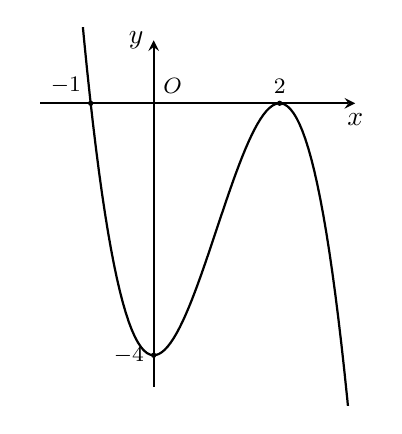
\begin{tikzpicture}[scale=0.8, >=stealth]
    \clip (-2.0, -4.8) rectangle (3.5, 1.2);
    \draw[->, line width=0.7pt] (-1.8, 0) -- (3.2, 0) node[below] {$x$};
    \draw[->, line width=0.7pt] (0, -4.5) -- (0, 1.0) node[left] {$y$};
    \node[above right, font=\footnotesize] at (0, 0) {$O$};

    % Điểm mốc trên trục
    \fill (-1, 0) circle (1.2pt) node[above left, font=\footnotesize] {$-1$};
    \fill (2, 0) circle (1.2pt) node[above, font=\footnotesize] {$2$};
    \fill (0, -4) circle (1.2pt) node[left, font=\footnotesize] {$-4$};

    % Đồ thị: y = -x^3 + 3x^2 - 4 tiếp xúc trục hoành tại x = 2, cực tiểu tại (0; -4), cắt Ox tại -1
    \draw[thick, domain=-1.2:3.5, samples=100] plot (\x, {-(\x)^3 + 3*(\x)^2 - 4});
\end{tikzpicture}
\end{center}
Xét tính đúng -- sai của các mệnh đề sau:}{
    \textbf{a)} & Hàm số đồng biến trên khoảng $(-4;2)$.
    & \textcolor{amberorange}{$\bigcirc$} & \textcolor{amberorange}{$\bigcirc$} \\ \hline
    
    \textbf{b)} & Hàm số đã cho có 2 điểm cực trị.
    & \textcolor{amberorange}{$\bigcirc$} & \textcolor{amberorange}{$\bigcirc$} \\ \hline
    
    \textbf{c)} & $d=-4$.
    & \textcolor{amberorange}{$\bigcirc$} & \textcolor{amberorange}{$\bigcirc$} \\ \hline
    
    \textbf{d)} & $a<0$, $b<0$, $c=0$.
    & \textcolor{amberorange}{$\bigcirc$} & \textcolor{amberorange}{$\bigcirc$} \\
}

% --- CÂU 15 (Tương ứng Câu 3 Phần II) ---
\questionTrueFalse{0}{15}{Cho hình chóp $S.ABCD$ có đáy là hình vuông cạnh $a$, $SA \perp (ABCD)$, $SA=3a$.
\begin{center}
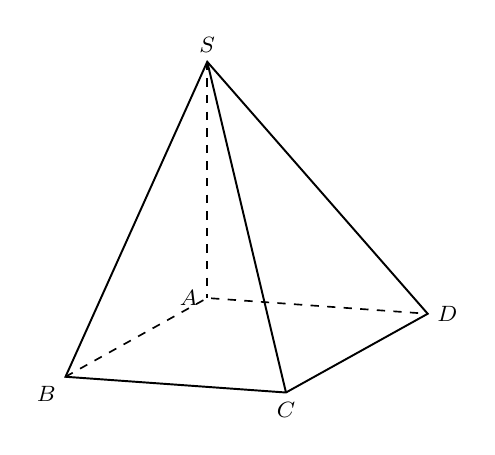
\begin{tikzpicture}[scale=1, >=stealth]
    \coordinate (A) at (1.8, 1.0);
    \coordinate (B) at (0, 0);
    \coordinate (C) at (2.8, -0.2);
    \coordinate (D) at (4.6, 0.8);
    \coordinate (S) at (1.8, 4.0);

    % Nét đứt
    \draw[dashed, line width=0.6pt] (B) -- (A) -- (D);
    \draw[dashed, line width=0.6pt] (S) -- (A);

    % Nét liền
    \draw[line width=0.7pt] (S) -- (B) -- (C) -- (D) -- cycle;
    \draw[line width=0.7pt] (S) -- (C);

    % Tên đỉnh
    \node[above, font=\footnotesize] at (S) {$S$};
    \node[left, font=\footnotesize] at (A) {$A$};
    \node[below left, font=\footnotesize] at (B) {$B$};
    \node[below, font=\footnotesize] at (C) {$C$};
    \node[right, font=\footnotesize] at (D) {$D$};
\end{tikzpicture}
\end{center}
Xét tính đúng -- sai của các mệnh đề sau:}{
    \textbf{a)} & $\vec{SA}+\vec{SC}=\vec{SB}+\vec{SD}$.
    & \textcolor{amberorange}{$\bigcirc$} & \textcolor{amberorange}{$\bigcirc$} \\ \hline
    
    \textbf{b)} & $\vec{SA}-\vec{SB}=\vec{SC}-\vec{SD}$.
    & \textcolor{amberorange}{$\bigcirc$} & \textcolor{amberorange}{$\bigcirc$} \\ \hline
    
    \textbf{c)} & $|\vec{AB}+\vec{SA}|=a\sqrt{10}$.
    & \textcolor{amberorange}{$\bigcirc$} & \textcolor{amberorange}{$\bigcirc$} \\ \hline
    
    \textbf{d)} & $\cos(\vec{AB},\vec{SC})=\dfrac{\sqrt{22}}{11}$.
    & \textcolor{amberorange}{$\bigcirc$} & \textcolor{amberorange}{$\bigcirc$} \\
}

% --- CÂU 16 (Tương ứng Câu 4 Phần II) ---
\questionTrueFalse{0}{16}{Một công ty sản xuất hàng may mặc, sản lượng đạt được tính bởi công thức sau:
\[ f(t)=\dfrac{3264t+2500}{2t} \]
với $f(t)$ là số sản phẩm (tính bằng bộ) và $t\ge0$ là thời gian (tính bằng ngày). Xét tính đúng -- sai của các mệnh đề sau:}{
    \textbf{a)} & Sản lượng đạt được vào ngày thứ 2 là 2250 bộ.
    & \textcolor{amberorange}{$\bigcirc$} & \textcolor{amberorange}{$\bigcirc$} \\ \hline
    
    \textbf{b)} & Sản lượng đạt được mỗi ngày càng ngày càng giảm theo thời gian.
    & \textcolor{amberorange}{$\bigcirc$} & \textcolor{amberorange}{$\bigcirc$} \\ \hline
    
    \textbf{c)} & Sản lượng đạt được mỗi ngày luôn lớn hơn 1650 bộ.
    & \textcolor{amberorange}{$\bigcirc$} & \textcolor{amberorange}{$\bigcirc$} \\ \hline
    
    \textbf{d)} & Chỉ tồn tại 2 điểm nằm trên đồ thị của hàm $f(t)$ sao cho mỗi điểm đều có hoành độ nguyên và khoảng cách từ mỗi điểm đó đến đường thẳng $y=-1632x$ lớn hơn $\sqrt{2}$.
    & \textcolor{amberorange}{$\bigcirc$} & \textcolor{amberorange}{$\bigcirc$} \\
}
\newpage

\textit{\textbf{PHẦN III. Câu trắc nghiệm trả lời ngắn. Thí sinh trả lời từ Câu 17 đến Câu 22.}}

\vspace{0.3cm}

% --- CÂU 17 (Tương ứng Câu 1 Phần III) ---
\questionShortAnswer{0}{17}{Cho hàm số $y=f(x)$ liên tục trên $\mathbb{R}\setminus\{1\}$ có bảng biến thiên như hình vẽ:
\begin{center}

\begin{tikzpicture}[scale=0.95]
    \tkzTabInit[lgt=1.2, espcl=2.2, deltacl=0.5]{$x$/0.8, $y'$/0.7, $y$/1.8}{$-\infty$, $-1$, $1$, $+\infty$}
    \tkzTabLine{, -, 0, +, d, +, }
    \tkzTabVar{+/$1$, -/$-\sqrt{2}$, +D-/$+\infty$/$-\infty$, +/$-1$}
\end{tikzpicture}
\end{center}
Tổng số đường tiệm cận đứng và đường tiệm cận ngang của đồ thị hàm số $y=f(x)$ là bao nhiêu?
}

% --- CÂU 18 (Tương ứng Câu 2 Phần III) ---
\questionShortAnswer{0}{18}{Giả sử doanh số (tính bằng số sản phẩm) của một sản phẩm mới (trong vòng một số năm nhất định) tuân theo quy luật logistic được mô hình hoá bằng hàm số $f(t)=\dfrac{3000}{1+3e^{-t}}$, $t\ge0$, trong đó thời gian $t$ được tính bằng năm, kể từ khi phát hành sản phẩm mới. Khi đó, đạo hàm $f'(t)$ sẽ biểu thị tốc độ bán hàng. Hỏi sau khi phát hành bao nhiêu năm thì tốc độ bán hàng là lớn nhất? (Kết quả được làm tròn đến hàng phần mười).
}

% --- CÂU 19 (Tương ứng Câu 3 Phần III) ---
\questionShortAnswer{0}{19}{Cho hàm số $y=f(x)$ liên tục, có đạo hàm trên $\mathbb{R}$. Đồ thị hàm số $y=f'(x)$ như hình vẽ bên. Hỏi hàm số $y=g(x)=f(x)-x$ có bao nhiêu điểm cực trị?
\begin{center}
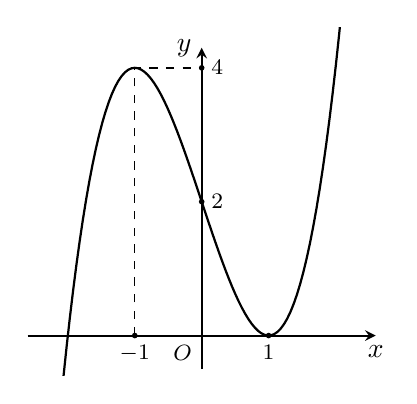
\begin{tikzpicture}[scale=0.85, >=stealth]
    \clip (-2.6, -0.6) rectangle (2.8, 4.6);
    \draw[->, line width=0.7pt] (-2.6, 0) -- (2.6, 0) node[below] {$x$};
    \draw[->, line width=0.7pt] (0, -0.5) -- (0, 4.3) node[left] {$y$};
    \node[below left, font=\footnotesize] at (0, 0) {$O$};

    \draw[dashed, line width=0.5pt] (-1, 0) -- (-1, 4) -- (0, 4);
    \fill (-1, 0) circle (1.2pt) node[below, font=\footnotesize] {$-1$};
    \fill (1, 0) circle (1.2pt) node[below, font=\footnotesize] {$1$};
    \fill (0, 2) circle (1.2pt) node[right, font=\footnotesize] {$2$};
    \fill (0, 4) circle (1.2pt) node[right, font=\footnotesize] {$4$};

    % Đồ thị f'(x) bậc 3: y = x^3 - 3x + 2
    \draw[thick, domain=-2.6:2.2, samples=100] plot (\x, {(\x)^3 - 3*(\x) + 2});
\end{tikzpicture}
\end{center}
}

% --- CÂU 20 (Tương ứng Câu 4 Phần III) ---
\questionShortAnswer{0}{20}{Cho một tấm tôn hình vuông cạnh $a = 240\text{ cm}$. Người ta cắt ở bốn góc tấm tôn bốn hình vuông bằng nhau, rồi gập tấm tôn lại để được một cái hộp không nắp để đựng nước.

\begin{center}
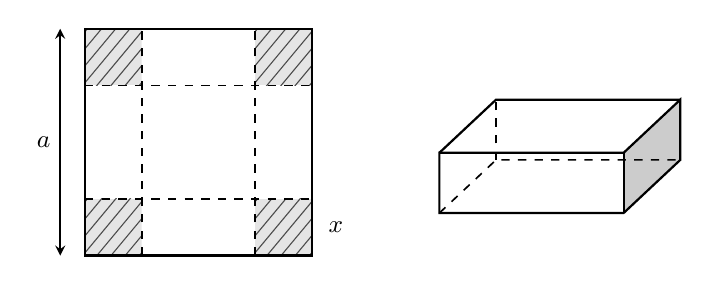
\begin{tikzpicture}[scale=0.9, >=stealth]
    % ==================== HÌNH 1: TẤM TÔN VUÔNG BỊ CẮT 4 GÓC ====================
    \begin{scope}[shift={(0,0)}]
        % Tô gạch chéo 4 góc hình vuông bị cắt
        \foreach \gx/\gy in {0/0, 2.4/0, 0/2.4, 2.4/2.4} {
            \begin{scope}
                \clip (\gx, \gy) rectangle (\gx+0.8, \gy+0.8);
                \fill[gray!20] (\gx, \gy) rectangle (\gx+0.8, \gy+0.8);
                \foreach \k in {-1.0, -0.8, ..., 2.0} {
                    \draw[black!70, line width=0.4pt] (\gx+\k, \gy-0.2) -- (\gx+\k+1.0, \gy+1.0);
                }
            \end{scope}
        }

        % Đường viền ngoài tấm tôn
        \draw[thick] (0,0) rectangle (3.2, 3.2);

        % Các đường nếp gấp (nét đứt)
        \draw[dashed, line width=0.6pt] (0.8, 0) -- (0.8, 3.2);
        \draw[dashed, line width=0.6pt] (2.4, 0) -- (2.4, 3.2);
        \draw[dashed, line width=0.6pt] (0, 0.8) -- (3.2, 0.8);
        \draw[dashed, line width=0.6pt] (0, 2.4) -- (3.2, 2.4);

        % Mũi tên chỉ kích thước cạnh a
        \draw[<->, line width=0.6pt] (-0.35, 0) -- (-0.35, 3.2);
        \node[left, font=\small] at (-0.35, 1.6) {$a$};

        % Ký hiệu độ dài x của góc cắt
        \node[right, font=\small] at (3.3, 0.4) {$x$};
    \end{scope}

    % ==================== HÌNH 2: HỘP KHÔNG NẮP ====================
    \begin{scope}[shift={(5.0, 0.6)}]
        % Tọa độ các đỉnh hộp chữ nhật
        \coordinate (A) at (0, 0);         % trước - trái - dưới
        \coordinate (B) at (2.6, 0);       % trước - phải - dưới
        \coordinate (C) at (3.4, 0.75);    % sau - phải - dưới
        \coordinate (D) at (0.8, 0.75);    % sau - trái - dưới

        \coordinate (A1) at (0, 0.85);      % trước - trái - trên
        \coordinate (B1) at (2.6, 0.85);    % trước - phải - trên
        \coordinate (C1) at (3.4, 1.6);     % sau - phải - trên
        \coordinate (D1) at (0.8, 1.6);     % sau - trái - trên

        % Mặt hông bên phải tô màu xám
        \fill[gray!40] (B) -- (C) -- (C1) -- (B1) -- cycle;

        % Nét khuất (đáy và góc sau)
        \draw[dashed, line width=0.6pt] (A) -- (D) -- (C);
        \draw[dashed, line width=0.6pt] (D) -- (D1);

        % Nét thấy (mặt trước, mặt hông và miệng hộp)
        \draw[thick] (A) -- (B) -- (C) -- (C1) -- (B1) -- (A1) -- cycle;
        \draw[thick] (B) -- (B1);
        \draw[thick] (A1) -- (D1) -- (C1);
    \end{scope}
\end{tikzpicture}
\end{center}

Trong các khối hộp tạo được, khối hộp có thể tích lớn nhất đựng được bao nhiêu lít nước? (với giả thiết các mép nối không đáng kể).
}

% --- CÂU 21 (Tương ứng Câu 5 Phần III) ---
\questionShortAnswer{0}{21}{Một chiếc ô tô được đặt trên mặt đáy dưới của một khung sắt có dạng hình hộp chữ nhật với đáy trên là hình chữ nhật $ABCD$. Mặt phẳng $(ABCD)$ song song với mặt phẳng nằm ngang. Khung sắt đó được buộc vào móc $E$ của chiếc cần cẩu sao cho các đoạn dây cáp $EA, EB, EC, ED$ có độ dài bằng nhau và cùng tạo với mặt phẳng $(ABCD)$ một góc bằng $60^{\circ}$. Chiếc cần cẩu kéo khung sắt lên theo phương thẳng đứng. Biết khối lượng của chiếc xe ô tô là $1256\text{ kg}$, trọng lượng của khung sắt là $3000\text{ N}$. Tính độ lớn các lực căng $\vec{F_1}, \vec{F_2}, \vec{F_3}, \vec{F_4}$ (Kết quả làm tròn đến hàng đơn vị), biết gia tốc trọng trường bằng $10\text{ m/s}^2$.
\begin{center}
    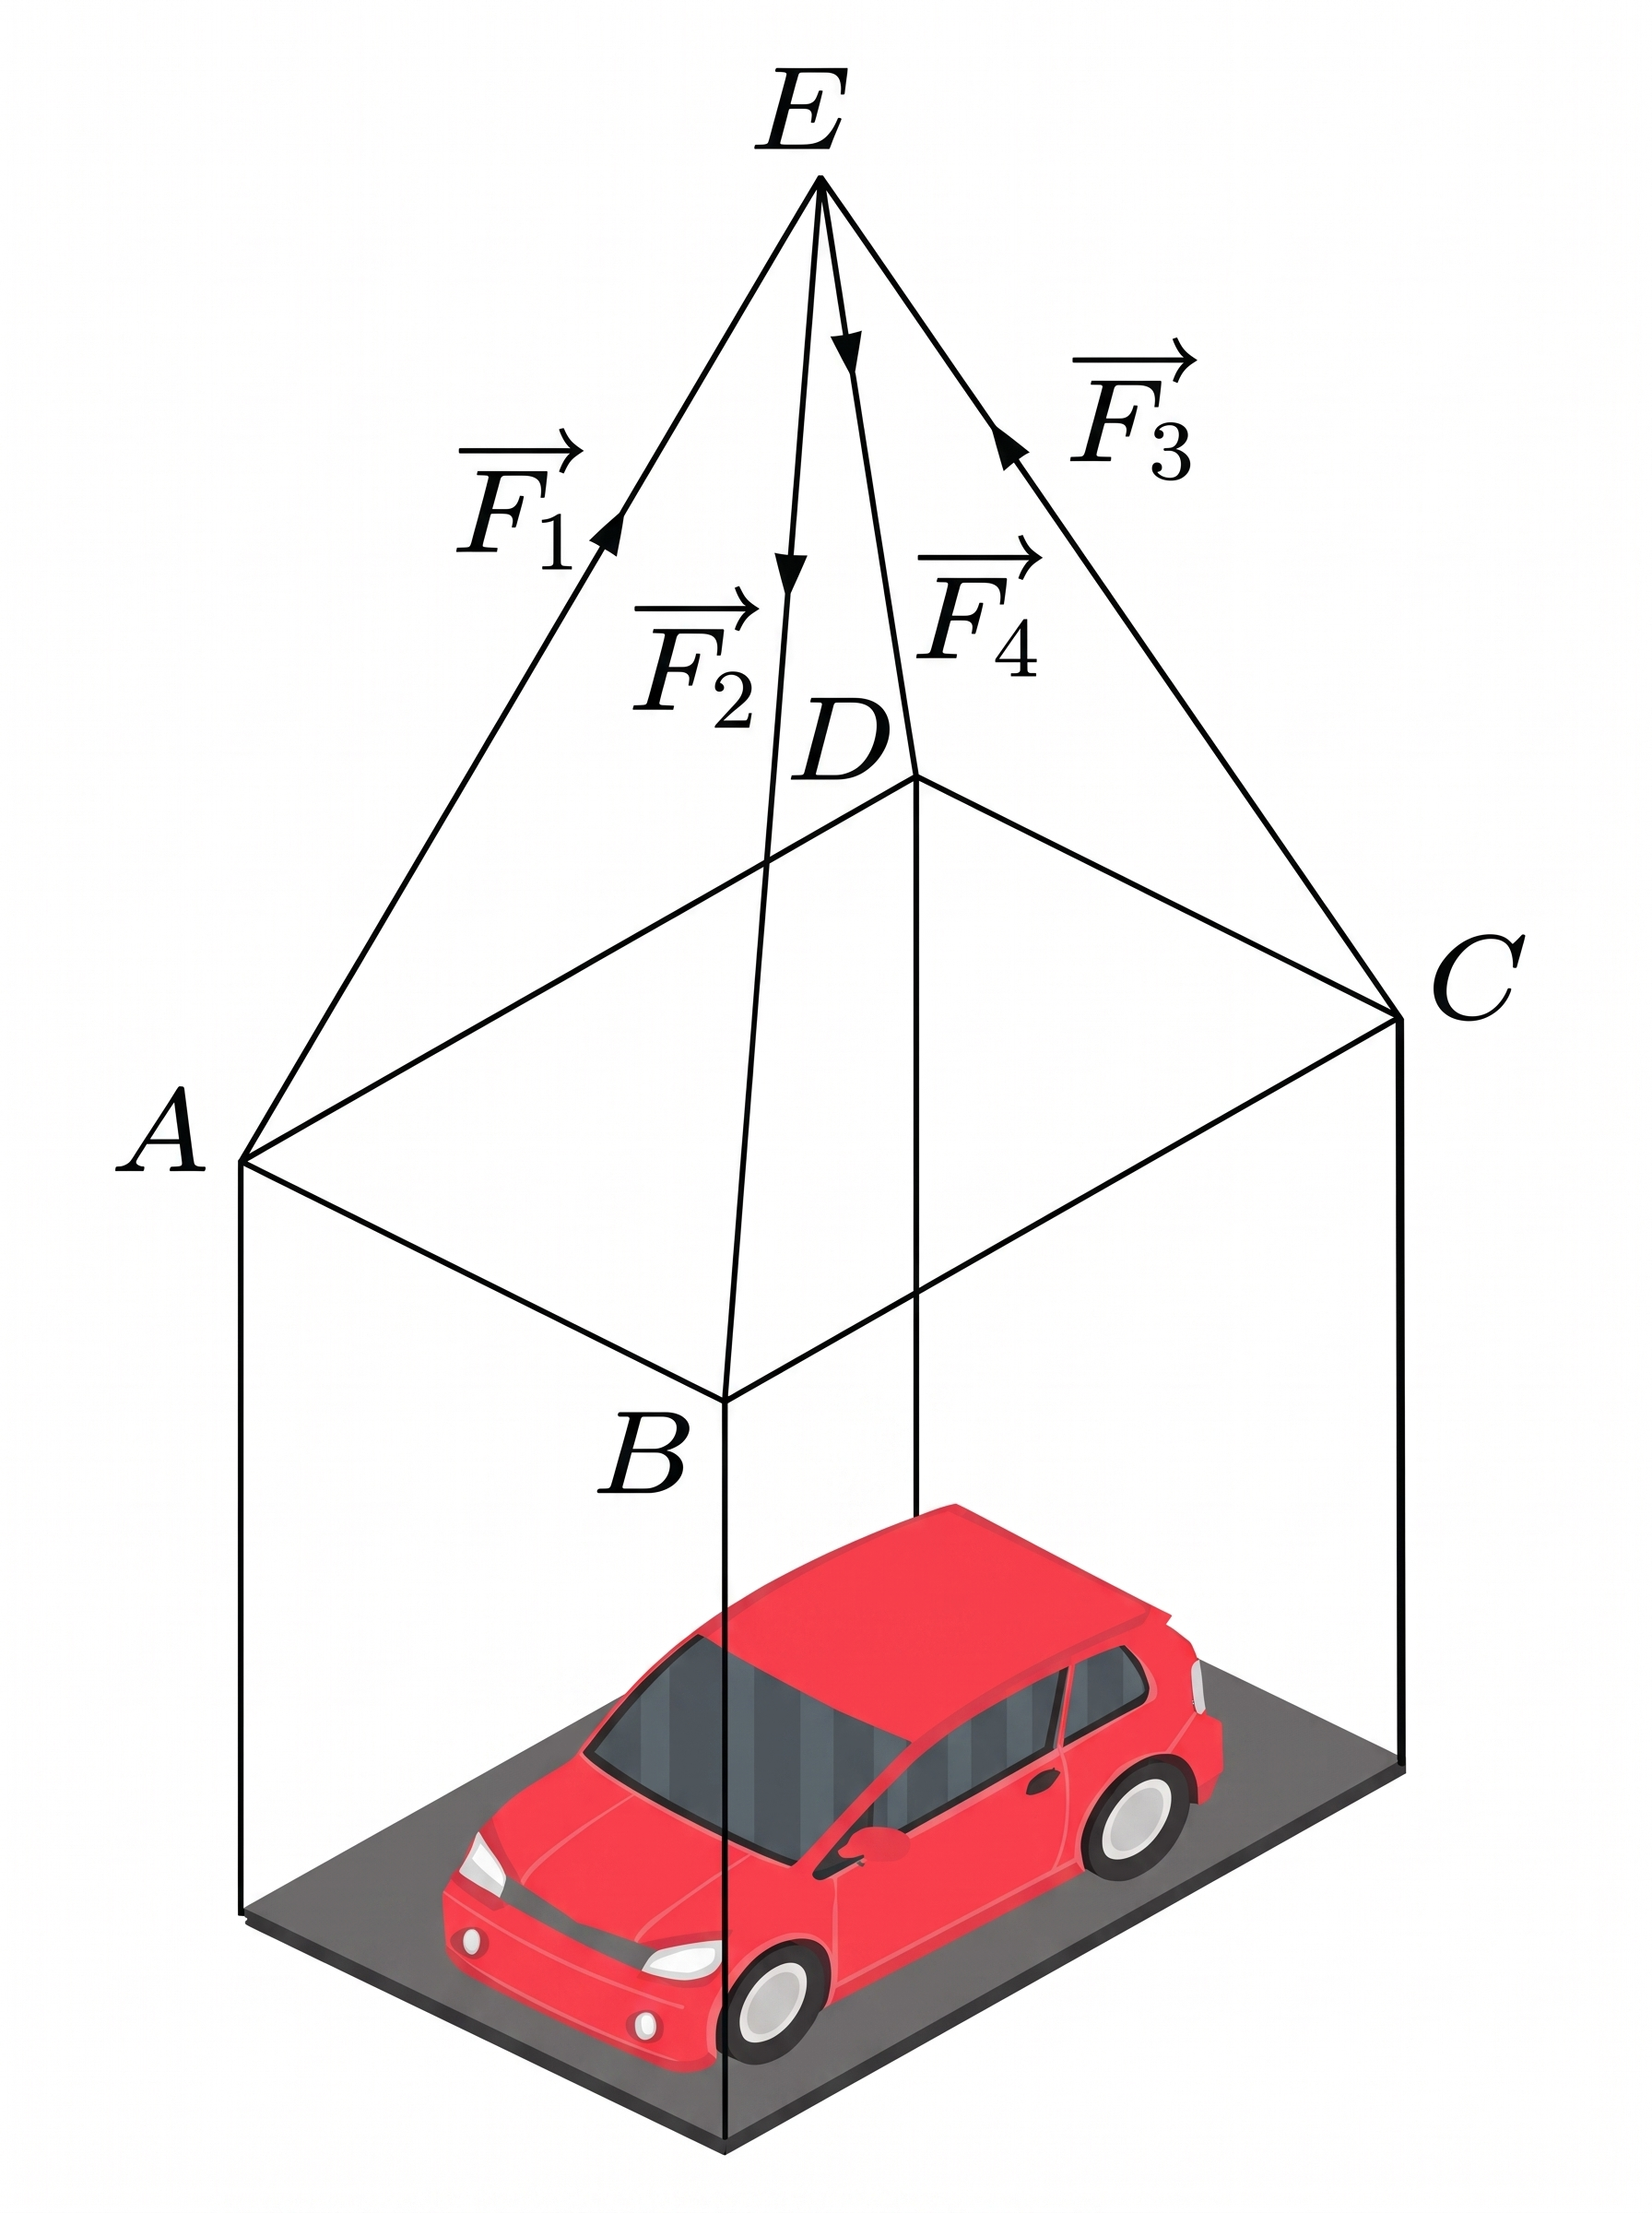
\includegraphics[width=0.25\textwidth]{Cau21.png}
\end{center}
}

% --- CÂU 22 (Tương ứng Câu 6 Phần III) ---
\questionShortAnswer{0}{22}{Cho hình lăng trụ $ABC.A'B'C'$. Gọi $M$ là trung điểm của $AC$, $N$ là một điểm thỏa mãn $\vec{BC}=3\vec{BN}$. Biết $\vec{MN}=x\vec{AB}+y\vec{AC}+z\vec{AA'}$. Giá trị của biểu thức $x+y+z$ bằng bao nhiêu?
}

\end{document}

% =========================================================================
% BẢNG ĐÁP ÁN THAM KHẢO CHO ĐỀ SỐ 3:
% =========================================================================
% PHẦN I:
% 1.C | 2.B | 3.C | 4.C | 5.A | 6.A | 7.A | 8.D | 9.B | 10.A | 11.B | 12.C
%
% PHẦN II:
% Câu 13 (Câu 1): a) Đúng | b) Sai  | c) Sai  | d) Đúng
% Câu 14 (Câu 2): a) Sai  | b) Đúng | c) Đúng | d) Sai
% Câu 15 (Câu 3): a) Đúng | b) Sai  | c) Đúng | d) Sai
% Câu 16 (Câu 4): a) Sai  | b) Đúng | c) Sai  | d) Sai
%
% PHẦN III:
% Câu 17 (Câu 1): 3
% Câu 18 (Câu 2): 1,1
% Câu 19 (Câu 3): 3
% Câu 20 (Câu 4): 1024
% Câu 21 (Câu 5): 4492
% Câu 22 (Câu 6): -0,5